\chapter{Quy hoạch động nâng cao}

\minitoc

\begin{baitap}{Trộn xâu}{https://oj.vnoi.info/problem/stmerge}

Cho 2 chuỗi $X$ gồm $N$ ký tự và $Y$ gồm $M$ ký tự.  

$X = X_1 X_2 \dots X_N$  

$Y = Y_1 Y_2 \dots Y_M$  \\

Hãy trộn 2 chuỗi $X$ và $Y$ này lại thành 1 chuỗi $T$ gồm $N + M$ ký tự sao cho vẫn bảo toàn được thứ tự xuất hiện của các ký tự trong 2 chuỗi.  

Ví dụ:  
$X = X_1 X_2$, $Y = Y_1 Y_2 Y_3$  

Một cách trộn hợp lệ: $T = X_1 Y_1 Y_2 X_2 Y_3$  \\

Xét 2 ký tự kề nhau $T[i], T[i+1]$:  
- Nếu chúng cùng thuộc $X$ hoặc cùng thuộc $Y$ thì chi phí cộng thêm là 0.  
- Nếu một thuộc $X$, một thuộc $Y$ thì chi phí cộng thêm là $cost[p][q]$ với $p, q$ tương ứng vị trí trong $X, Y$.  

\textbf{Input}
\begin{itemize}[noitemsep]
    \item Dòng đầu tiên chứa số $Q$ – số bộ dữ liệu.
    \item Mỗi test:  
    \begin{itemize}
        \item Dòng đầu tiên chứa hai số $N, M$ $(1 \leq N, M \leq 10^3)$.
        \item Dòng tiếp theo chứa $M$ số nguyên – $cost[1][j]$ với $j = 1..M$.
        \item $N-1$ dòng tiếp theo, mỗi dòng chứa $M$ số nguyên – các giá trị $cost[i][j]$ $(1 \leq i \leq N, 1 \leq j \leq M)$.
    \end{itemize}
\end{itemize}

\textbf{Output}  
Với mỗi test, in ra chi phí nhỏ nhất để trộn.

\textbf{Ví dụ}

\begin{sampleio}
1 & 6 \\
2 3 & \\
3 2 30 & \\
15 5 4 & \\
\end{sampleio}

\end{baitap}


\textbf{Phân tích bài toán}

Gọi $f[i][j][k]$ là tổng chi phí nhỏ nhất khi trộn $X[1..i]$ và $Y[1..j]$
\begin{itemize}
    \item $k = 0$: ký tự cuối cùng thuộc chuỗi $X$
    \item $k = 1$: ký tự cuối cùng thuộc chuỗi $Y$
\end{itemize} 

\textbf{Trường hợp cơ sở:}
\begin{itemize}
    \item $f[1][0][0] = 0$
    \item $f[0][1][1] = 0$
    \item $f[i][0][0] = 0$, $\forall i \geq 2$
    \item $f[0][j][1] = 0$, $\forall j \geq 2$
\end{itemize}

\textbf{Kết quả bài toán:} $\min(f[M][N][0], f[M][N][1])$\\

Xét $X[1..i]$ và $Y[1..j]$, nếu ký tự cuối cùng thuộc $X$, ta có 2 trường hợp xảy ra:

\begin{itemize}
    \item $f[i][j][0] = f[i - 1][j][1] + cost[i][j]$ : Chuyển từ $Y$ sang $X$ 
    \item $f[i][j][0] = f[i - 1][j][0] + 0$ : Chuyển từ $X$ sang $X$.
\end{itemize}
    
Ngược lại nếu ký tự cuối cùng thuộc $Y$, ta có 2 trường hợp xảy ra:
\begin{itemize}
    \item $f[i][j][1] = f[i][j - 1][0] + cost[i][j]$ : Chuyển từ $X$ sang $Y$
    \item $f[i][j][1] = f[i][j - 1][1] + 0$ : Chuyển từ $Y$ sang $Y$
\end{itemize}

Từ những phân tích trên, ta rút ra được công thức truy hồi tổng quát:


\[
f[i][j][k] = \min \Big( 
    \begin{cases}
        f[i - (k == 0)][j - (k == 1)][k], \\
        f[i - (k == 0)][j - (k == 1)][1 - k] + cost[i][j]
    \end{cases}
    \Big)
\]


\begin{lstlisting}[title=\centering\textbf{Cài đặt}]
#include <bits/stdc++.h>
#define int long long
const int oo = 1e18 + 7;
using namespace std;

signed main() {
    int q; cin >> q;
    while (q--) {
        int m, n; cin >> m >> n;
        vector<vector<int>> cost(m + 1, vector<int>(n + 1));
        for (int i = 1; i <= m; i++) {
            for (int j = 1; j <= n; j++) {
                cin >> cost[i][j];
            }
        }

        vector<vector<vector<int>>> f(m + 1, vector<vector<int>>(n + 1, vector<int>(2, oo)));

        for (int i = 1; i <= m; i++) {
            f[i][0][0] = 0;
        }
        for (int j = 1; j <= n; j++) {
            f[0][j][1] = 0;
        }

        for (int i = 1; i <= m; i++) {
            for (int j = 1; j <= n; j++) {
                f[i][j][0] = min(f[i - 1][j][0], f[i - 1][j][1] + cost[i][j]);

                f[i][j][1] = min(f[i][j - 1][1], f[i][j - 1][0] + cost[i][j]);
            }
        }
        cout << min(f[m][n][0], f[m][n][1]) << endl;
    }
}
\end{lstlisting}


\begin{baitap}{Trò chơi với băng số}{https://oj.vnoi.info/problem/linegame}

Có một băng số gồm $n$ ô vuông, đánh số từ 1 đến $n$.  
Ô vuông thứ $i$ ghi một số nguyên dương $a_i$.  

Trong một lượt chơi, người tham gia chọn một dãy các ô $(i_1, i_2, \dots, i_k)$ theo thứ tự từ trái sang phải.  
Điểm số thu được là:
\[
a_{i_1} - a_{i_2} + a_{i_3} - a_{i_4} + \dots + (-1)^{k-1} a_{i_k}
\]

Hãy tính số điểm lớn nhất có thể đạt được từ một lượt chơi.

\textbf{Input}
\begin{itemize}[noitemsep]
    \item Dòng đầu tiên chứa số $n$ $(1 \leq n \leq 10^6)$.
    \item Dòng thứ hai chứa $n$ số nguyên $a_i$ $(1 \leq a_i \leq 10^4)$.
\end{itemize}

\textbf{Output}  
In ra số điểm lớn nhất có thể đạt được.

\textbf{Ví dụ}

\begin{sampleio}
7 & 17 \\
4 9 2 4 1 3 7 & \\
\end{sampleio}

\begin{figure}[h]
    \centering
    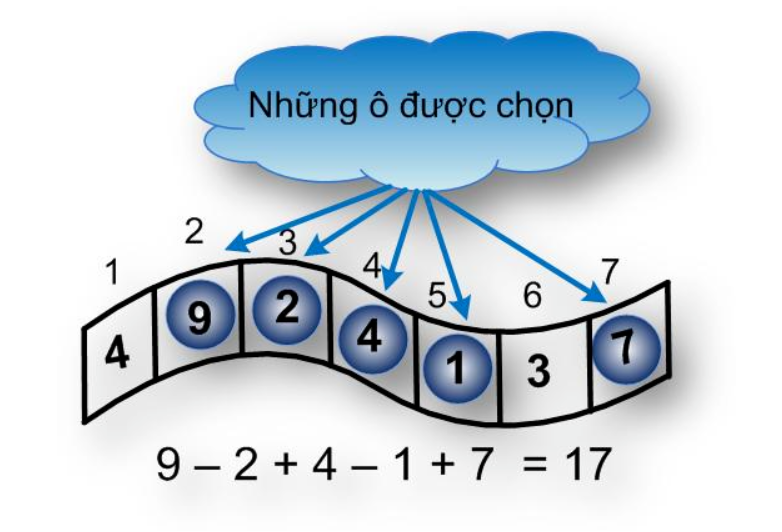
\includegraphics[width=0.4\textwidth]{resource/img/linegame.png}
    \caption{Hình minh họa bài toán.}
\end{figure}

\end{baitap}
\textbf{Phân tích bài toán}  

Gọi $f[i][k]$ là số điểm lớn nhất có thể đạt được khi xét $i$ ô đầu tiên:  
\begin{itemize}
    \item $k = 0$: ô $i$ được chọn và đóng vai trò dấu $+$.
    \item $k = 1$: ô $i$ được chọn và đóng vai trò dấu $-$.
\end{itemize}

\textbf{Trường hợp cơ sở:} $f[1][0] = a[1], \quad f[1][1] = -a[1], \quad f[0][0] = f[0][1] = 0$.\\

\textbf{Kết quả bài toán:}  $\max(f[n][0],\ f[n][1])$\\

Xét ô $i$, ta có các lựa chọn như sau:

\begin{itemize}
    \item Nếu $k = 0$ (ô $i$ mang dấu $+$):
    \begin{itemize}
        \item Nối tiếp từ trạng thái trước đó có dấu $-$: $f[i][0] = f[i-1][1] + a[i]$.
        \item Bắt đầu một dãy mới tại ô $i$: $f[i][0] = a[i]$.
        \item Bỏ qua ô $i$: $f[i][0] = f[i-1][0]$.
    \end{itemize}
    Vậy: $f[i][0] = \max \big( f[i-1][1] + a[i],\ a[i],\ f[i-1][0] \big)$

    \item Nếu $k = 1$ (ô $i$ mang dấu $-$):
    \begin{itemize}
        \item Nối tiếp từ trạng thái trước đó có dấu $+$: $f[i][1] = f[i-1][0] - a[i]$.
        \item Bắt đầu một dãy mới tại ô $i$: $f[i][1] = -a[i]$.
        \item Bỏ qua ô $i$: $f[i][1] = f[i-1][1]$.
    \end{itemize}
    Vậy: $f[i][1] = \max \big( f[i-1][0] - a[i],\ -a[i],\ f[i-1][1] \big)$
\end{itemize}


\begin{lstlisting}[title=\centering\textbf{Cài đặt}]
#include <bits/stdc++.h>
#define int long long
using namespace std;
const int oo = 1e18 + 7;

signed main() {
    int n; cin >> n;
    vector<int> a(n + 1);
    for (int i = 1; i <= n; i++) {
        cin >> a[i];
    }
    vector<vector<int>> f(n + 1, vector<int>(2, -oo));
    f[1][0] = a[1];
    f[0][0] = 0;

    for (int i = 1; i <= n; i++) {
        f[i][0] = max(f[i][0], a[i]);
        f[i][0] = max(f[i][0], f[i - 1][0]);
        f[i][0] = max(f[i][0], f[i - 1][1] + a[i]);
        
        f[i][1] = max(f[i][1], f[i - 1][1]);
        f[i][1] = max(f[i][1], f[i - 1][0] - a[i]);
    }

    int ans = -oo;

    for (int i = 1; i <= n; i++) {
        ans = max({ans,f[i][0], f[i][1]});
    }
    cout << ans;
}
\end{lstlisting}


\begin{baitap}{Two Paths}{https://lqdoj.edu.vn/problem/twopaths}

Hai anh em An và Bình tham gia một trò chơi thám hiểm trên bảng số \textbf{xTremeMaze}.  

Bảng có kích thước $N \times M$ ($N$ dòng và $M$ cột).  
Mỗi ô $(i,j)$ chứa một số nguyên (có thể âm hoặc dương) biểu diễn điểm kinh nghiệm nhận được khi đi vào ô đó.  

An và Bình bắt đầu tại ô $(1,1)$ và kết thúc tại ô $(N,M)$.  
Mỗi lượt, một người chỉ được đi xuống hoặc sang phải, và không được đi ra ngoài bảng.  
Điểm kinh nghiệm tại ô $(1,1)$ và $(N,M)$ luôn bằng $0$.  

Yêu cầu: tìm tổng điểm kinh nghiệm lớn nhất mà hai anh em đạt được, với điều kiện hai người không đi qua cùng một ô, ngoại trừ ô $(1,1)$ và ô $(N,M)$.

\textbf{Input}
\begin{itemize}[noitemsep]
    \item Dòng đầu tiên chứa hai số nguyên $N, M$ $(2 \leq N, M \leq 200)$.
    \item $N$ dòng tiếp theo, mỗi dòng chứa $M$ số nguyên có giá trị tuyệt đối không quá $100$ — điểm kinh nghiệm của từng ô. 
    \item Bảo đảm $A_{1,1} = A_{N,M} = 0$.
\end{itemize}

\textbf{Output}  
In ra tổng số điểm kinh nghiệm lớn nhất mà An và Bình đạt được.

\textbf{Ví dụ}

\begin{sampleio}
3 3 & 32 \\
0 2 3 & \\
4 5 6 & \\
7 8 0 & \\
\end{sampleio}
\end{baitap}

\textbf{Phân tích bài toán}

Gọi $f[\text{step}][x_1][x_2]$ là tổng số điểm kinh nghiệm lớn nhất khi An và Bình đã thực hiện  
$\text{step} = x + y - 2$ bước, trong đó:
\begin{itemize}
    \item An đang ở vị trí $(x_1, y_1)$ với $y_1 = \text{step} - x_1 + 2$,
    \item Bình đang ở vị trí $(x_2, y_2)$ với $y_2 = \text{step} - x_2 + 2$.
\end{itemize}

Tổng số bước di chuyển là $n + m - 2$, do đó ta duyệt lần lượt các bước $\text{step} = 1 \rightarrow n + m - 2$.

\textbf{Trường hợp cơ sở:} $f[0][1][1] = 0$\\

\textbf{Kết quả bài toán:} $f[n + m - 2][n][n]$\\

\textbf{Công thức truy hồi:}  
Tại mỗi bước, giá trị $f[\text{step}][x_1][x_2]$ được cập nhật từ 4 trạng thái trước đó, ứng với việc An/Bình đi xuống hoặc sang phải:
\[
\begin{aligned}
f[\text{step}][x_1][x_2] = \max \Big\{ 
   & f[\text{step} - 1][x_1 - 1][x_2 - 1], \\
   & f[\text{step} - 1][x_1 - 1][x_2], \\
   & f[\text{step} - 1][x_1][x_2 - 1], \\
   & f[\text{step} - 1][x_1][x_2] 
\Big\} + \text{điểm}
\end{aligned}
\]

Trong đó phần \textit{điểm} được tính như sau:
\[
\text{nếu } (x_1, y_1) = (x_2, y_2) \Rightarrow \text{điểm} = a[x_1][y_1]
\]
\[
\text{ngược lại } \Rightarrow \text{điểm} = a[x_1][y_1] + a[x_2][y_2]
\]

Ngoài ra, cần đảm bảo các điều kiện sau:
\begin{itemize}
    \item $(x_1, y_1)$ và $(x_2, y_2)$ phải nằm trong bảng.
    \item Nếu $(x_1, y_1) = (x_2, y_2)$ thì đó chỉ có thể là ô đích $(n,m)$.
\end{itemize}


\begin{lstlisting}[title=\centering\textbf{Cài đặt}]
#include <bits/stdc++.h>
#define int long long
const int oo = 1e9 + 7;
using namespace std;


signed main() {
    int n, m; cin >> n >> m;
    vector<vector<int>> a(n + 1, vector<int>(m + 1));
    for (int i = 1; i <= n; i++) {
        for (int j = 1; j <= m; j++) {
            cin >> a[i][j];
        }
    }

    vector<vector<vector<int>>> f(n + m, vector<vector<int>>(n + 1, vector<int>(n + 1, -oo)));

    f[0][1][1] = 0;

    for (int step = 1; step <= n + m - 2; step++) {
        for (int x1 = 1; x1 <= n; x1++) {
            int y1 = step - x1 + 2;
            if (y1 <= 0 || y1 > m) continue;
            for (int x2 = 1; x2 <= n; x2++) {
                int y2 = step - x2 + 2;
                if (y2 <= 0 || y2 > m) continue;

                int val = -oo;
                val = max(val, f[step - 1][x1 - 1][x2]);
                val = max(val, f[step - 1][x1][x2 - 1]);
                val = max(val, f[step - 1][x1 - 1][x2 - 1]);
                val = max(val, f[step - 1][x1][x2]); 


                if (x1 == x2 && y1 == y2 && (x1 != n || y1 != m)) continue;

                if (x1 == x2 && y1 == y2)
                    val += a[x1][y1];
                else
                    val += a[x1][y1] + a[x2][y2];
                f[step][x1][x2] = val;
            }
        }
    }
    cout << f[n + m - 2][n][n];
}
\end{lstlisting}

\begin{baitap}{IOI07 Miners}{https://oj.vnoi.info/problem/nkminers}

Có hai mỏ than, mỗi mỏ có một nhóm thợ mỏ làm việc. Khai thác than là công việc vất vả, do đó các thợ mỏ cần thực phẩm để hoạt động. Mỗi khi một đợt vận chuyển thực phẩm đến mỏ, các thợ mỏ sẽ khai thác được một lượng than nào đó. Có 3 loại thực phẩm được vận chuyển: thịt (M), cá (F) và bánh mì (B).

Mỗi đợt vận chuyển thực phẩm được đưa đến một trong hai mỏ, và sản lượng than của đợt đó phụ thuộc vào số loại thực phẩm khác nhau trong hai đợt liên tiếp mà mỏ đó nhận được:
\begin{itemize}
    \item Nếu các đợt vận chuyển cùng một loại thực phẩm $\Rightarrow$ 1 đơn vị than
    \item Nếu có 2 loại thực phẩm khác nhau $\Rightarrow$ 2 đơn vị than
    \item Nếu có 3 loại thực phẩm khác nhau $\Rightarrow$ 3 đơn vị than
\end{itemize}

Các đợt vận chuyển không thể chia nhỏ, và tất cả thực phẩm trong một đợt phải gửi đến một trong hai mỏ. Có thể gửi tất cả các đợt đến một mỏ.

Hãy tìm cách phân chia các đợt vận chuyển sao cho tổng lượng than khai thác được từ hai mỏ là lớn nhất.

\textbf{Input}
\begin{itemize}[noitemsep]
    \item Dòng đầu tiên chứa số nguyên $N$ $(1 \leq N \leq 10^5)$ — số đợt vận chuyển.
    \item Dòng thứ hai chứa xâu $S$ độ dài $N$, mỗi ký tự là một trong \{M, F, B\}.
\end{itemize}

\textbf{Output}  
In ra tổng lượng than lớn nhất có thể khai thác.

\textbf{Ví dụ}

\begin{sampleio}
6 & 12 \\
MBMFFB & \\ \hline
16 & 29 \\
MMBMBBBBMMMMMBMB & \\
\end{sampleio}
\end{baitap}

\textbf{Phân tích bài toán}

Gọi $f[i][a_1][a_2][b_1][b_2]$ là tổng lượng than lớn nhất có thể sản xuất được sau $i$ đợt vận chuyển, trong đó:
\begin{itemize}
    \item $a_1, a_2$ là hai loại thực phẩm gần nhất mỏ 1 đã nhận (Hiện tại là $a_1$, ngày hôm trước là $a_2$).
    \item $b_1, b_2$ là hai loại thực phẩm gần nhất mỏ 2 đã nhận (Hiện tại là $b_1$, ngày hôm trước là $b_2$).
    \item Giá trị của mỗi loại: $0$ (không có), $1$ (M), $2$ (F), $3$ (B).
\end{itemize}

\textbf{Trường hợp cơ sở:}

Giả sử thực phẩm đầu tiên là loại $t = \texttt{code}(s[1])$, ta có:
\begin{align*}
f[1][t][0][0][0] &= 1 \quad \text{(gửi đến mỏ 1)} \\
f[1][0][0][t][0] &= 1 \quad \text{(gửi đến mỏ 2)}
\end{align*}

\textbf{Kết quả bài toán:} 
\[
\max_{a,b,c,d \in \{0,1,2,3\}} f[n][a][b][c][d]
\]

Với $i \geq 2$, giả sử loại thực phẩm hiện tại là $c = \texttt{code}(s[i])$, ta có hai lựa chọn:

\begin{itemize}
    \item \textbf{Chuyển đến mỏ 1}:
    \[
    f[i][c][a_1][b_1][b_2] = \max(f[i][c][a_1][b_1][b_2], f[i - 1][a_1][a_2][b_1][b_2] + \texttt{energy}(c, a_1, a_2))
    \]

    \item \textbf{Chuyển đến mỏ 2}:
    \[
    f[i][a_1][a_2][c][b_1] = \max(f[i][a_1][a_2][c][b_1], f[i - 1][a_1][a_2][b_1][b_2] + \texttt{energy}(c, b_1, b_2))
    \]
\end{itemize}

Trong đó, hàm \texttt{energy}(a, b, c) là hàm đếm số loại thực phẩm khác nhau trong 3 ngày gần nhất:
\[
\texttt{energy}(a, b, c) = \left| \{a, b, c\} \setminus \{0\} \right|
\]


\begin{lstlisting}[title=\centering\textbf{Cài đặt}]
#include <bits/stdc++.h>
#define int long long
const int oo = 1e9 + 7;
using namespace std;

int code(char c) {
    return (c == 'M' ? 1 : (c == 'F' ? 2 : (c == 'B' ? 3 : 0)));
}

int energy(int a, int b, int c) {
    return (a != 0) + (b != 0 && b != a) + (c != 0 && c != a && c != b);
}

signed main() {
    ios_base::sync_with_stdio(0); 
    cin.tie(0), cout.tie(0);
    int n; cin >> n;
    vector<char> s(n + 1);
    for (int i = 1; i <= n; i++) cin >> s[i];

    int f[n + 1][4][4][4][4];
    for (int i = 0; i <= n; i++)
        for (int a1 = 0; a1 < 4; a1++)
            for (int a2 = 0; a2 < 4; a2++)
                for (int b1 = 0; b1 < 4; b1++)
                    for (int b2 = 0; b2 < 4; b2++)
                        f[i][a1][a2][b1][b2] = -oo;

    int t = code(s[1]);
    f[1][t][0][0][0] = 1;
    f[1][0][0][t][0] = 1;

    for (int i = 2; i <= n; i++) {
        int cur = code(s[i]);
        for (int t1 = 0; t1 <= 3; t1++) {
            for (int t2 = 0; t2 <= 3; t2++) {
                for (int t3 = 0; t3 <= 3; t3++) {
                    for (int t4 = 0; t4 <= 3; t4++) {
                        f[i][cur][t1][t3][t4] = max(f[i][cur][t1][t3][t4],
                                                    f[i - 1][t1][t2][t3][t4] + energy(cur, t1,t2));
                        
                        f[i][t1][t2][cur][t3] = max(f[i][t1][t2][cur][t3],
                                                    f[i - 1][t1][t2][t3][t4] + energy(cur,t3,t4));
                    }
                }
            }
        }
    }


    int ans = 0;
    for (int a1 = 0; a1 < 4; ++a1)
        for (int a2 = 0; a2 < 4; ++a2)
            for (int b1 = 0; b1 < 4; ++b1)
                for (int b2 = 0; b2 < 4; ++b2)
                    ans = max(ans, f[n][a1][a2][b1][b2]);
    cout << ans;
}
\end{lstlisting}

\textbf{Phân tích bài toán (2):}

Gọi $f[i][a][b][c]$ là tổng lượng than lớn nhất có thể sản xuất được sau $i$ đợt vận chuyển, trong đó:
\begin{itemize}
    \item Mỏ vừa nhận đợt $i$ (gọi là mỏ \textit{đang hoạt động}) có hai loại thực phẩm gần nhất là $(s[i], a)$, tức $s[i]$ là loại hiện tại, $a$ là loại liền trước đó.
    \item Mỏ còn lại có hai loại thực phẩm gần nhất là $(b, c)$.
    \item Giá trị của mỗi loại: $0$ (không có), $1$ (M), $2$ (F), $3$ (B).
\end{itemize}

\textbf{Trường hợp cơ sở:}

Với đợt vận chuyển đầu tiên có loại $t = \texttt{code}(s[1])$, ta có: $f[1][0][0][0] = 1$
vì $\texttt{energy}(t,0,0) = 1$.


\textbf{Kết quả bài toán:} 
\[
\max_{a,b,c \in \{0,1,2,3\}} f[n][a][b][c]
\]


\textbf{Công thức chuyển:}

Giả sử ở đợt $i$ hiện tại loại thực phẩm là $c = \texttt{code}(s[i])$, khi xét đến đợt tiếp theo $s[i+1]$ có loại $t = \texttt{code}(s[i+1])$, ta có hai lựa chọn:

\begin{itemize}
    \item \textbf{Tiếp tục chuyển đến mỏ đang hoạt động}:  
    Khi đó hai món gần nhất của mỏ này là $(s[i], a)$, nên điểm cộng thêm là $\texttt{energy}(t, s[i], a)$.  
    Trạng thái mới ở bước $i+1$ sẽ là:
    \[
    f[i+1][s[i]][b][c] = \max\Big(f[i+1][s[i]][b][c],\; f[i][a][b][c] + \texttt{energy}(t, s[i], a)\Big)
    \]

    \item \textbf{Chuyển sang mỏ còn lại}:  
    Mỏ còn lại hiện có hai món gần nhất là $(b, c)$, nên điểm cộng thêm là $\texttt{energy}(t, b, c)$.  
    Sau khi giao, mỏ này trở thành mỏ đang hoạt động với $(t, b)$, còn mỏ cũ trở thành mỏ còn lại với $(s[i], a)$.  
    Do đó:
    \[
    f[i+1][b][s[i]][a] = \max\Big(f[i+1][b][s[i]][a],\; f[i][a][b][c] + \texttt{energy}(t, b, c)\Big)
    \]
\end{itemize}



\begin{lstlisting}[title=\centering\textbf{Cài đặt}]
#include <bits/stdc++.h>
using namespace std;
const int oo = 1e9 + 7;

int code(char c) {
    return (c == 'M' ? 1 : (c == 'F' ? 2 : (c == 'B' ? 3 : 0)));
}

int energy(int a, int b, int c) {
    return (a != 0) + (b != 0 && b != a) + (c != 0 && c != a && c != b);
}

int main() {
    ios_base::sync_with_stdio(0); 
    cin.tie(0), cout.tie(0);
    int n; cin >> n;
    vector<char> s(n + 1);
    for (int i = 1; i <= n; i++) cin >> s[i];

    int f[n + 1][4][4][4];
    for (int i = 0; i <= n; i++) 
        for (int a = 0; a < 4; a++)
            for (int b = 0; b < 4; b++) 
                for (int c = 0; c < 4; c++)
                    f[i][a][b][c] = -1;
                    
    f[0][0][0][0] = 0;
    f[1][0][0][0] = 1;  
    for (int i = 0; i < n; i++) {
        for (int a = 0; a < 4; a++) {
            for (int b = 0; b < 4; b++) {
                for (int c = 0; c < 4; c++) {
                    if (f[i][a][b][c] == -1) continue;

                    f[i + 1][code(s[i])][b][c] = max(f[i + 1][code(s[i])][b][c], f[i][a][b][c] + energy(code(s[i]), code(s[i + 1]), a));

                    f[i + 1][b][code(s[i])][a] = max(f[i + 1][b][code(s[i])][a], f[i][a][b][c] + energy(code(s[i+1]), b, c));

                }
            }
        }
    }

    int ans = 0;
    for (int a = 0; a < 4; a++) {
        for (int b = 0; b < 4; b++) {
            for (int c = 0; c < 4; c++) {
                ans = max(ans, f[n][a][b][c]);
            }
        }
    }
    cout << ans;
}
\end{lstlisting}
